
%% bare_conf_compsoc.tex
%% V1.4b
%% 2015/08/26
%% by Michael Shell
%% See:
%% http://www.michaelshell.org/
%% for current contact information.
%%
%% This is a skeleton file demonstrating the use of IEEEtran.cls
%% (requires IEEEtran.cls version 1.8b or later) with an IEEE Computer
%% Society conference paper.
%%
%% Support sites:
%% http://www.michaelshell.org/tex/ieeetran/
%% http://www.ctan.org/pkg/ieeetran
%% and
%% http://www.ieee.org/

%%*************************************************************************
%% Legal Notice:
%% This code is offered as-is without any warranty either expressed or
%% implied; without even the implied warranty of MERCHANTABILITY or
%% FITNESS FOR A PARTICULAR PURPOSE! 
%% User assumes all risk.
%% In no event shall the IEEE or any contributor to this code be liable for
%% any damages or losses, including, but not limited to, incidental,
%% consequential, or any other damages, resulting from the use or misuse
%% of any information contained here.
%%
%% All comments are the opinions of their respective authors and are not
%% necessarily endorsed by the IEEE.
%%
%% This work is distributed under the LaTeX Project Public License (LPPL)
%% ( http://www.latex-project.org/ ) version 1.3, and may be freely used,
%% distributed and modified. A copy of the LPPL, version 1.3, is included
%% in the base LaTeX documentation of all distributions of LaTeX released
%% 2003/12/01 or later.
%% Retain all contribution notices and credits.
%% ** Modified files should be clearly indicated as such, including  **
%% ** renaming them and changing author support contact information. **
%%*************************************************************************


% *** Authors should verify (and, if needed, correct) their LaTeX system  ***
% *** with the testflow diagnostic prior to trusting their LaTeX platform ***
% *** with production work. The IEEE's font choices and paper sizes can   ***
% *** trigger bugs that do not appear when using other class files.       ***                          ***
% The testflow support page is at:
% http://www.michaelshell.org/tex/testflow/



\documentclass[conference,compsoc]{IEEEtran}
% Some/most Computer Society conferences require the compsoc mode option,
% but others may want the standard conference format.
%
% If IEEEtran.cls has not been installed into the LaTeX system files,
% manually specify the path to it like:
% \documentclass[conference,compsoc]{../sty/IEEEtran}





% Some very useful LaTeX packages include:
% (uncomment the ones you want to load)


% *** MISC UTILITY PACKAGES ***
%
%\usepackage{ifpdf}
% Heiko Oberdiek's ifpdf.sty is very useful if you need conditional
% compilation based on whether the output is pdf or dvi.
% usage:
% \ifpdf
%   % pdf code
% \else
%   % dvi code
% \fi
% The latest version of ifpdf.sty can be obtained from:
% http://www.ctan.org/pkg/ifpdf
% Also, note that IEEEtran.cls V1.7 and later provides a builtin
% \ifCLASSINFOpdf conditional that works the same way.
% When switching from latex to pdflatex and vice-versa, the compiler may
% have to be run twice to clear warning/error messages.






% *** CITATION PACKAGES ***
%
\ifCLASSOPTIONcompsoc
  % IEEE Computer Society needs nocompress option
  % requires cite.sty v4.0 or later (November 2003)
  \usepackage[nocompress]{cite}
\else
  % normal IEEE
  \usepackage{cite}
\fi
% cite.sty was written by Donald Arseneau
% V1.6 and later of IEEEtran pre-defines the format of the cite.sty package
% \cite{} output to follow that of the IEEE. Loading the cite package will
% result in citation numbers being automatically sorted and properly
% "compressed/ranged". e.g., [1], [9], [2], [7], [5], [6] without using
% cite.sty will become [1], [2], [5]--[7], [9] using cite.sty. cite.sty's
% \cite will automatically add leading space, if needed. Use cite.sty's
% noadjust option (cite.sty V3.8 and later) if you want to turn this off
% such as if a citation ever needs to be enclosed in parenthesis.
% cite.sty is already installed on most LaTeX systems. Be sure and use
% version 5.0 (2009-03-20) and later if using hyperref.sty.
% The latest version can be obtained at:
% http://www.ctan.org/pkg/cite
% The documentation is contained in the cite.sty file itself.
%
% Note that some packages require special options to format as the Computer
% Society requires. In particular, Computer Society  papers do not use
% compressed citation ranges as is done in typical IEEE papers
% (e.g., [1]-[4]). Instead, they list every citation separately in order
% (e.g., [1], [2], [3], [4]). To get the latter we need to load the cite
% package with the nocompress option which is supported by cite.sty v4.0
% and later.





% *** GRAPHICS RELATED PACKAGES ***
%
\ifCLASSINFOpdf
  % \usepackage[pdftex]{graphicx}
  % declare the path(s) where your graphic files are
  % \graphicspath{{../pdf/}{../jpeg/}}
  % and their extensions so you won't have to specify these with
  % every instance of \includegraphics
  % \DeclareGraphicsExtensions{.pdf,.jpeg,.png}
\else
  % or other class option (dvipsone, dvipdf, if not using dvips). graphicx
  % will default to the driver specified in the system graphics.cfg if no
  % driver is specified.
  % \usepackage[dvips]{graphicx}
  % declare the path(s) where your graphic files are
  % \graphicspath{{../eps/}}
  % and their extensions so you won't have to specify these with
  % every instance of \includegraphics
  % \DeclareGraphicsExtensions{.eps}
\fi
% graphicx was written by David Carlisle and Sebastian Rahtz. It is
% required if you want graphics, photos, etc. graphicx.sty is already
% installed on most LaTeX systems. The latest version and documentation
% can be obtained at: 
% http://www.ctan.org/pkg/graphicx
% Another good source of documentation is "Using Imported Graphics in
% LaTeX2e" by Keith Reckdahl which can be found at:
% http://www.ctan.org/pkg/epslatex
%
% latex, and pdflatex in dvi mode, support graphics in encapsulated
% postscript (.eps) format. pdflatex in pdf mode supports graphics
% in .pdf, .jpeg, .png and .mps (metapost) formats. Users should ensure
% that all non-photo figures use a vector format (.eps, .pdf, .mps) and
% not a bitmapped formats (.jpeg, .png). The IEEE frowns on bitmapped formats
% which can result in "jaggedy"/blurry rendering of lines and letters as
% well as large increases in file sizes.
%
% You can find documentation about the pdfTeX application at:
% http://www.tug.org/applications/pdftex





% *** MATH PACKAGES ***
%
%\usepackage{amsmath}
% A popular package from the American Mathematical Society that provides
% many useful and powerful commands for dealing with mathematics.
%
% Note that the amsmath package sets \interdisplaylinepenalty to 10000
% thus preventing page breaks from occurring within multiline equations. Use:
%\interdisplaylinepenalty=2500
% after loading amsmath to restore such page breaks as IEEEtran.cls normally
% does. amsmath.sty is already installed on most LaTeX systems. The latest
% version and documentation can be obtained at:
% http://www.ctan.org/pkg/amsmath





% *** SPECIALIZED LIST PACKAGES ***
%
%\usepackage{algorithmic}
% algorithmic.sty was written by Peter Williams and Rogerio Brito.
% This package provides an algorithmic environment fo describing algorithms.
% You can use the algorithmic environment in-text or within a figure
% environment to provide for a floating algorithm. Do NOT use the algorithm
% floating environment provided by algorithm.sty (by the same authors) or
% algorithm2e.sty (by Christophe Fiorio) as the IEEE does not use dedicated
% algorithm float types and packages that provide these will not provide
% correct IEEE style captions. The latest version and documentation of
% algorithmic.sty can be obtained at:
% http://www.ctan.org/pkg/algorithms
% Also of interest may be the (relatively newer and more customizable)
% algorithmicx.sty package by Szasz Janos:
% http://www.ctan.org/pkg/algorithmicx




% *** ALIGNMENT PACKAGES ***
%
%\usepackage{array}
% Frank Mittelbach's and David Carlisle's array.sty patches and improves
% the standard LaTeX2e array and tabular environments to provide better
% appearance and additional user controls. As the default LaTeX2e table
% generation code is lacking to the point of almost being broken with
% respect to the quality of the end results, all users are strongly
% advised to use an enhanced (at the very least that provided by array.sty)
% set of table tools. array.sty is already installed on most systems. The
% latest version and documentation can be obtained at:
% http://www.ctan.org/pkg/array


% IEEEtran contains the IEEEeqnarray family of commands that can be used to
% generate multiline equations as well as matrices, tables, etc., of high
% quality.




% *** SUBFIGURE PACKAGES ***
%\ifCLASSOPTIONcompsoc
%  \usepackage[caption=false,font=footnotesize,labelfont=sf,textfont=sf]{subfig}
%\else
%  \usepackage[caption=false,font=footnotesize]{subfig}
%\fi
% subfig.sty, written by Steven Douglas Cochran, is the modern replacement
% for subfigure.sty, the latter of which is no longer maintained and is
% incompatible with some LaTeX packages including fixltx2e. However,
% subfig.sty requires and automatically loads Axel Sommerfeldt's caption.sty
% which will override IEEEtran.cls' handling of captions and this will result
% in non-IEEE style figure/table captions. To prevent this problem, be sure
% and invoke subfig.sty's "caption=false" package option (available since
% subfig.sty version 1.3, 2005/06/28) as this is will preserve IEEEtran.cls
% handling of captions.
% Note that the Computer Society format requires a sans serif font rather
% than the serif font used in traditional IEEE formatting and thus the need
% to invoke different subfig.sty package options depending on whether
% compsoc mode has been enabled.
%
% The latest version and documentation of subfig.sty can be obtained at:
% http://www.ctan.org/pkg/subfig




% *** FLOAT PACKAGES ***
%
%\usepackage{fixltx2e}
% fixltx2e, the successor to the earlier fix2col.sty, was written by
% Frank Mittelbach and David Carlisle. This package corrects a few problems
% in the LaTeX2e kernel, the most notable of which is that in current
% LaTeX2e releases, the ordering of single and double column floats is not
% guaranteed to be preserved. Thus, an unpatched LaTeX2e can allow a
% single column figure to be placed prior to an earlier double column
% figure.
% Be aware that LaTeX2e kernels dated 2015 and later have fixltx2e.sty's
% corrections already built into the system in which case a warning will
% be issued if an attempt is made to load fixltx2e.sty as it is no longer
% needed.
% The latest version and documentation can be found at:
% http://www.ctan.org/pkg/fixltx2e


%\usepackage{stfloats}
% stfloats.sty was written by Sigitas Tolusis. This package gives LaTeX2e
% the ability to do double column floats at the bottom of the page as well
% as the top. (e.g., "\begin{figure*}[!b]" is not normally possible in
% LaTeX2e). It also provides a command:
%\fnbelowfloat
% to enable the placement of footnotes below bottom floats (the standard
% LaTeX2e kernel puts them above bottom floats). This is an invasive package
% which rewrites many portions of the LaTeX2e float routines. It may not work
% with other packages that modify the LaTeX2e float routines. The latest
% version and documentation can be obtained at:
% http://www.ctan.org/pkg/stfloats
% Do not use the stfloats baselinefloat ability as the IEEE does not allow
% \baselineskip to stretch. Authors submitting work to the IEEE should note
% that the IEEE rarely uses double column equations and that authors should try
% to avoid such use. Do not be tempted to use the cuted.sty or midfloat.sty
% packages (also by Sigitas Tolusis) as the IEEE does not format its papers in
% such ways.
% Do not attempt to use stfloats with fixltx2e as they are incompatible.
% Instead, use Morten Hogholm'a dblfloatfix which combines the features
% of both fixltx2e and stfloats:
%
% \usepackage{dblfloatfix}
% The latest version can be found at:
% http://www.ctan.org/pkg/dblfloatfix




% *** PDF, URL AND HYPERLINK PACKAGES ***
%
%\usepackage{url}
% url.sty was written by Donald Arseneau. It provides better support for
% handling and breaking URLs. url.sty is already installed on most LaTeX
% systems. The latest version and documentation can be obtained at:
% http://www.ctan.org/pkg/url
% Basically, \url{my_url_here}.




% *** Do not adjust lengths that control margins, column widths, etc. ***
% *** Do not use packages that alter fonts (such as pslatex).         ***
% There should be no need to do such things with IEEEtran.cls V1.6 and later.
% (Unless specifically asked to do so by the journal or conference you plan
% to submit to, of course. )


% correct bad hyphenation here
\hyphenation{op-tical net-works semi-conduc-tor}
\usepackage{graphicx}
\graphicspath{ {./images/} }

\usepackage[hyphens]{url}
\usepackage{hyperref}
\hyphenation{op-tical net-works semi-conduc-tor}

\setlength{\parskip}{1em}

\begin{document}
%
% paper title
% Titles are generally capitalized except for words such as a, an, and, as,
% at, but, by, for, in, nor, of, on, or, the, to and up, which are usually
% not capitalized unless they are the first or last word of the title.
% Linebreaks \\ can be used within to get better formatting as desired.
% Do not put math or special symbols in the title.
\title{Creating a Virtual Piano with Leap Motion Technology}


% author names and affiliations
% use a multiple column layout for up to three different
% affiliations
\author{\IEEEauthorblockN{Rebecca Kopacz}
\IEEEauthorblockA{Computer Science Department\\
Colorado State University\\
Fort Collins, CO\\
rkopacz@rams.colostate.edu}
\and
\IEEEauthorblockN{Morgan VandeRiet}
\IEEEauthorblockA{Computer Science Department\\
Colorado State University\\
Fort Collins, CO\\
mvanderi@rams.colostate.edu}}

% conference papers do not typically use \thanks and this command
% is locked out in conference mode. If really needed, such as for
% the acknowledgment of grants, issue a \IEEEoverridecommandlockouts
% after \documentclass

% for over three affiliations, or if they all won't fit within the width
% of the page (and note that there is less available width in this regard for
% compsoc conferences compared to traditional conferences), use this
% alternative format:
% 
%\author{\IEEEauthorblockN{Michael Shell\IEEEauthorrefmark{1},
%Homer Simpson\IEEEauthorrefmark{2},
%James Kirk\IEEEauthorrefmark{3}, 
%Montgomery Scott\IEEEauthorrefmark{3} and
%Eldon Tyrell\IEEEauthorrefmark{4}}
%\IEEEauthorblockA{\IEEEauthorrefmark{1}School of Electrical and Computer Engineering\\
%Georgia Institute of Technology,
%Atlanta, Georgia 30332--0250\\ Email: see http://www.michaelshell.org/contact.html}
%\IEEEauthorblockA{\IEEEauthorrefmark{2}Twentieth Century Fox, Springfield, USA\\
%Email: homer@thesimpsons.com}
%\IEEEauthorblockA{\IEEEauthorrefmark{3}Starfleet Academy, San Francisco, California 96678-2391\\
%Telephone: (800) 555--1212, Fax: (888) 555--1212}
%\IEEEauthorblockA{\IEEEauthorrefmark{4}Tyrell Inc., 123 Replicant Street, Los Angeles, California 90210--4321}}




% use for special paper notices
%\IEEEspecialpapernotice{(Invited Paper)}




% make the title area
\maketitle

% As a general rule, do not put math, special symbols or citations
% in the abstract
\begin{abstract}
With advancements in technology in the recent decades, almost all aspects of life have obtained a virtual form, especially with the recent COVID-19 pandemic. As a society, we have found a way to do almost all of our activities online, including learning. Music technology and education has taken a new shape as virtual instruments can oftentimes be more convenient and cost effective. This paper discusses the creation of a virtual piano that can be played with the Leap Motion controller. It will discuss previous research in virtual instruments, the creation of the virtual piano, a research study of the project, and potential future work.
\end{abstract}

\begin{IEEEkeywords}
Leap Motion, music technology, technological piano, Unity, virtual learning.
\end{IEEEkeywords}




% For peer review papers, you can put extra information on the cover
% page as needed:
% \ifCLASSOPTIONpeerreview
% \begin{center} \bfseries EDICS Category: 3-BBND \end{center}
% \fi
%
% For peerreview papers, this IEEEtran command inserts a page break and
% creates the second title. It will be ignored for other modes.
\IEEEpeerreviewmaketitle



\section{Introduction}
% no \IEEEPARstart

The rise of gestural recognition platforms have given way to new opportunities of musical instruments. Using newer technologies, we have begun to explore potential improvements to the existing virtual instrument field, where users can interact with realistic instruments without the need for one.
Ultraleap's Leap Motion controller, an optical hand tracker, is one of these technologies that have allowed the creation of new interactive virtual instruments.

Our team has created a virtual piano that can be played using the Leap Motion device. Users hold their hands above the controller which sits flat on the table in front of the computer keyboard. The user's hand movements are reflected onto the computer screen where they can interact with the virtual piano. This project has the potential to create interactive tools with an abundance of uses including music education, medical rehabilitation, and the replacement of a real piano.

Since the start of the COVID-19 pandemic more than a year ago, virtual programs are now required more than ever. Schools continue to teach online which has greatly impacted the way music is taught. Many students no longer have access to real instruments which can greatly impact the effectiveness of their learning. Teachers have resorted to showing videos which are less effective than hands on learning. This project could allow students to continue learning about music while still remaining in a virtual environment.

\begin{figure}[h]
\centering
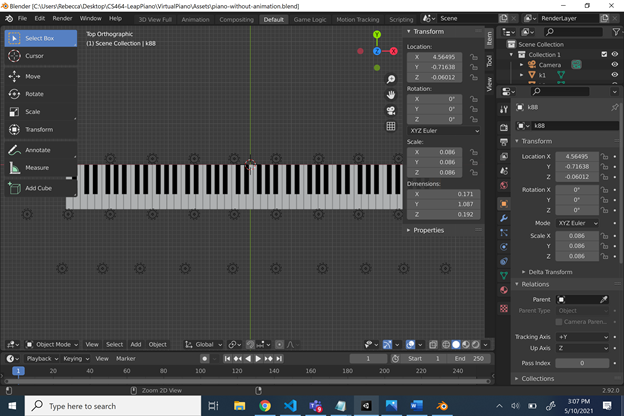
\includegraphics[width=7cm, height=4cm]{IEEEtran/Picture2.png}
\centering
\caption{This is the model developed by a previous group in Blender. We have added additional components in Unity to create the virtual piano. Image taken by Kopacz and VandeRiet.}
\end{figure}

Interactive tools provide more opportunities for education, and virtual musical instruments can be the perfect tool for music education. The virtual piano is significantly cheaper than any other option currently on the market. They are also smaller, portable, and have the potential to include a multitude of instruments students might not usually have access to. These benefits could allow schools to stock their music rooms with many instruments at a fraction of the cost. Teachers and students would be able to have more resources readily available to use at their discretion.

Additionally, gestural based technology and Virtual Reality (VR) have become increasingly helpful tools within the medical industry. One of the uses of this technology, is within rehabilitation and physical therapy. Patients are able to incorporate their entire bodies which allows them to recuperate in a new and improved way. "Within Medicine, VR has been used in teaching anatomy, training
in diagnostic procedures (such as virtual colonoscopy, or virtual
bronchroscopy), teaching open and minimally-invasive surgery
procedures, and in rehabilitation," [19]. While a virtual piano may not be a necessary tool for most medical needs, the base technology is a potential tool that could contribute to the development of medical related VR programs and rehabilitation.

% An example of a floating figure using the graphicx package.
% Note that \label must occur AFTER (or within) \caption.
% For figures, \caption should occur after the \includegraphics.
% Note that IEEEtran v1.7 and later has special internal code that
% is designed to preserve the operation of \label within \caption
% even when the captionsoff option is in effect. However, because
% of issues like this, it may be the safest practice to put all your
% \label just after \caption rather than within \caption{}.
%
% Reminder: the "draftcls" or "draftclsnofoot", not "draft", class
% option should be used if it is desired that the figures are to be
% displayed while in draft mode.
%
%\begin{figure}[!t]
%\centering
%\includegraphics[width=2.5in]{myfigure}
% where an .eps filename suffix will be assumed under latex, 
% and a .pdf suffix will be assumed for pdflatex; or what has been declared
% via \DeclareGraphicsExtensions.
%\caption{Simulation results for the network.}
%\label{fig_sim}
%\end{figure}

% Note that the IEEE typically puts floats only at the top, even when this
% results in a large percentage of a column being occupied by floats.


% An example of a double column floating figure using two subfigures.
% (The subfig.sty package must be loaded for this to work.)
% The subfigure \label commands are set within each subfloat command,
% and the \label for the overall figure must come after \caption.
% \hfil is used as a separator to get equal spacing.
% Watch out that the combined width of all the subfigures on a 
% line do not exceed the text width or a line break will occur.
%
%\begin{figure*}[!t]
%\centering
%\subfloat[Case I]{\includegraphics[width=2.5in]{box}%
%\label{fig_first_case}}
%\hfil
%\subfloat[Case II]{\includegraphics[width=2.5in]{box}%
%\label{fig_second_case}}
%\caption{Simulation results for the network.}
%\label{fig_sim}
%\end{figure*}
%
% Note that often IEEE papers with subfigures do not employ subfigure
% captions (using the optional argument to \subfloat[]), but instead will
% reference/describe all of them (a), (b), etc., within the main caption.
% Be aware that for subfig.sty to generate the (a), (b), etc., subfigure
% labels, the optional argument to \subfloat must be present. If a
% subcaption is not desired, just leave its contents blank,
% e.g., \subfloat[].


% An example of a floating table. Note that, for IEEE style tables, the
% \caption command should come BEFORE the table and, given that table
% captions serve much like titles, are usually capitalized except for words
% such as a, an, and, as, at, but, by, for, in, nor, of, on, or, the, to
% and up, which are usually not capitalized unless they are the first or
% last word of the caption. Table text will default to \footnotesize as
% the IEEE normally uses this smaller font for tables.
% The \label must come after \caption as always.
%
%\begin{table}[!t]
%% increase table row spacing, adjust to taste
%\renewcommand{\arraystretch}{1.3}
% if using array.sty, it might be a good idea to tweak the value of
% \extrarowheight as needed to properly center the text within the cells
%\caption{An Example of a Table}
%\label{table_example}
%\centering
%% Some packages, such as MDW tools, offer better commands for making tables
%% than the plain LaTeX2e tabular which is used here.
%\begin{tabular}{|c||c|}
%\hline
%One & Two\\
%\hline
%Three & Four\\
%\hline
%\end{tabular}
%\end{table}


% Note that the IEEE does not put floats in the very first column
% - or typically anywhere on the first page for that matter. Also,
% in-text middle ("here") positioning is typically not used, but it
% is allowed and encouraged for Computer Society conferences (but
% not Computer Society journals). Most IEEE journals/conferences use
% top floats exclusively. 
% Note that, LaTeX2e, unlike IEEE journals/conferences, places
% footnotes above bottom floats. This can be corrected via the
% \fnbelowfloat command of the stfloats package.
\section{Background}
The introduction of gesture based interaction and new input technologies have given rise to many new forms of Human-Computer interaction, including the debut of digital based musical instruments. Electronic music has become an increasingly popular development in the last few decades, though it is not new technology. One early example of electronic music is the Theremin invented in 1919. This instrument was also gesture based as it was played by moving one’s hands between two metal antennas to control frequency (pitch) and amplitude (volume). Recent developments in digital musical instruments enjoy increasingly more user interfaces. Touch screen and Virtual Reality (VR) devices are just some of the many interfaces that have allowed for advancements in the music industry.

With more sophisticated gesture based technologies, the world of digital musical instruments is growing. Now, technologies can better emulate playing a real instrument without actually needing one. Devices like Microsoft’s Kinect, Nintendo’s Wii, and Virtual Reality headsets have opened doors for an even wider range of possibilities. The Nintendo Wii remote’s debut in 2006 allowed for many cost effective experiments including, the “Wiiolin” [9], a virtual violin that could be played by moving the Wii’s sensor bar over the Wii remote. Another example is the ChromaChord, which uses an Oculus Rift headset and Leap Motion controller. The leap motion controller, made by UltraLeap, is an optical hand tracking module which captures the movements of the user’s hands. The device plugs into the computer’s USB port and sits flat on the table in front of the keyboard. Users hover their hands about six inches over the device, and the leap motion will imitate the hand motions onto the screen. The device has little to no noticeable latency, allowing the user to comfortably play without frustration. This system allows a performer to play single notes and chords [15]. Developing virtual reality musical instruments such as the Wiiolin and the ChromaChord is a challenge, but they are extremely beneficial to the continuous growth of human computer interaction.

\begin{figure}[h]
\centering
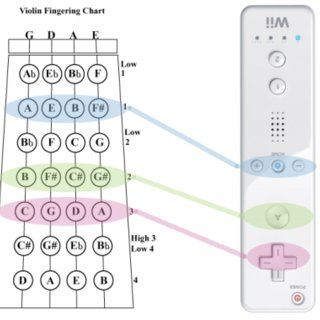
\includegraphics[width=5cm, height=6cm]{IEEEtran/Wiiolin.jpg}
\centering
\caption{This is an image that describes how the "Wiiolin" works. This image is by Tracy Anne Hammond on reasearchgate.net. Found using a public domain.}
\end{figure}

Others areas of technology in music have been studied including tempo, latency, and precision with instruments. In 2011, as multi-touch surfaces became increasingly popular, Montag, Sullivan, Dickey and Leider explored the effects of audio latency and how it provided a negative experience to any kind of musical technology using the interface. They then created a multi-touch table that uses a system output that simultaneously drives the audio display and the haptic display, resulting in no latency between audio and haptic feedback systems. Performance context and behavior were also studied in relation to the analysis of digital musical instruments and new interfaces to do so [11].

While many musical technologies have emerged, virtual teaching devices for music are still in the early stages of development. “[M]ost instrument implementations in VR are simple string or tapping based instruments,” [14]. The more complicated an instrument is, the harder it is to develop it as a virtual reality musical instrument. Camera-based motion tracking is a common technology used with musical interfaces and human computer interaction. It utilizes cameras and infrared sensors to “see” a person’s motion [2]. The use of wearable technology, such as data gloves, is another popular way of determining the gestures of humans. It is effective with the detection of joint angles and other orientations of the body [2]. 

One combined approach, of camera-based motion and wearable technology, is the Leap Motion tool. The Leap Motion “is a USB peripheral designed to create an invisible air space surrounding a computer screen that can be interacted with,” [13]. Since its development in 2013, the Leap Motion has contributed a lot to musical interfaces and human computer interaction. Unlike the Xbox Kinect and other similar systems, the Leap Motion is capable of tracking larger movements and more precise gestures. It is a groundbreaking device that is a widespread tool for any interface of musical expression.

The Leap Motion and other technological systems have contributed a lot to the development of virtual reality musical instruments, but they are also important to other human computer interaction activities. However, unlike other activities, “music seems to involve almost aloof the brain,” [6]. It can involve the whole body, not just the mind, which is vital to those suffering from Alzheimer’s and other diseases. Music helps people to engage their bodies and minds. The combination of both music and body movement can really help with rehabilitation for many patients.

The piano is one musical instrument that has been created into a virtual reality musical instrument many times. Augmented reality (AR) has played an important part in the development of piano teaching techniques. “The application of augmented reality technology in teaching has great potential, which can optimize the presentation effect of teaching materials and promote the interaction between teachers and students in class,” [7]. Although the piano has been recreated virtually several times, there is always a need for more improvement.

\begin{figure}[h]
\centering
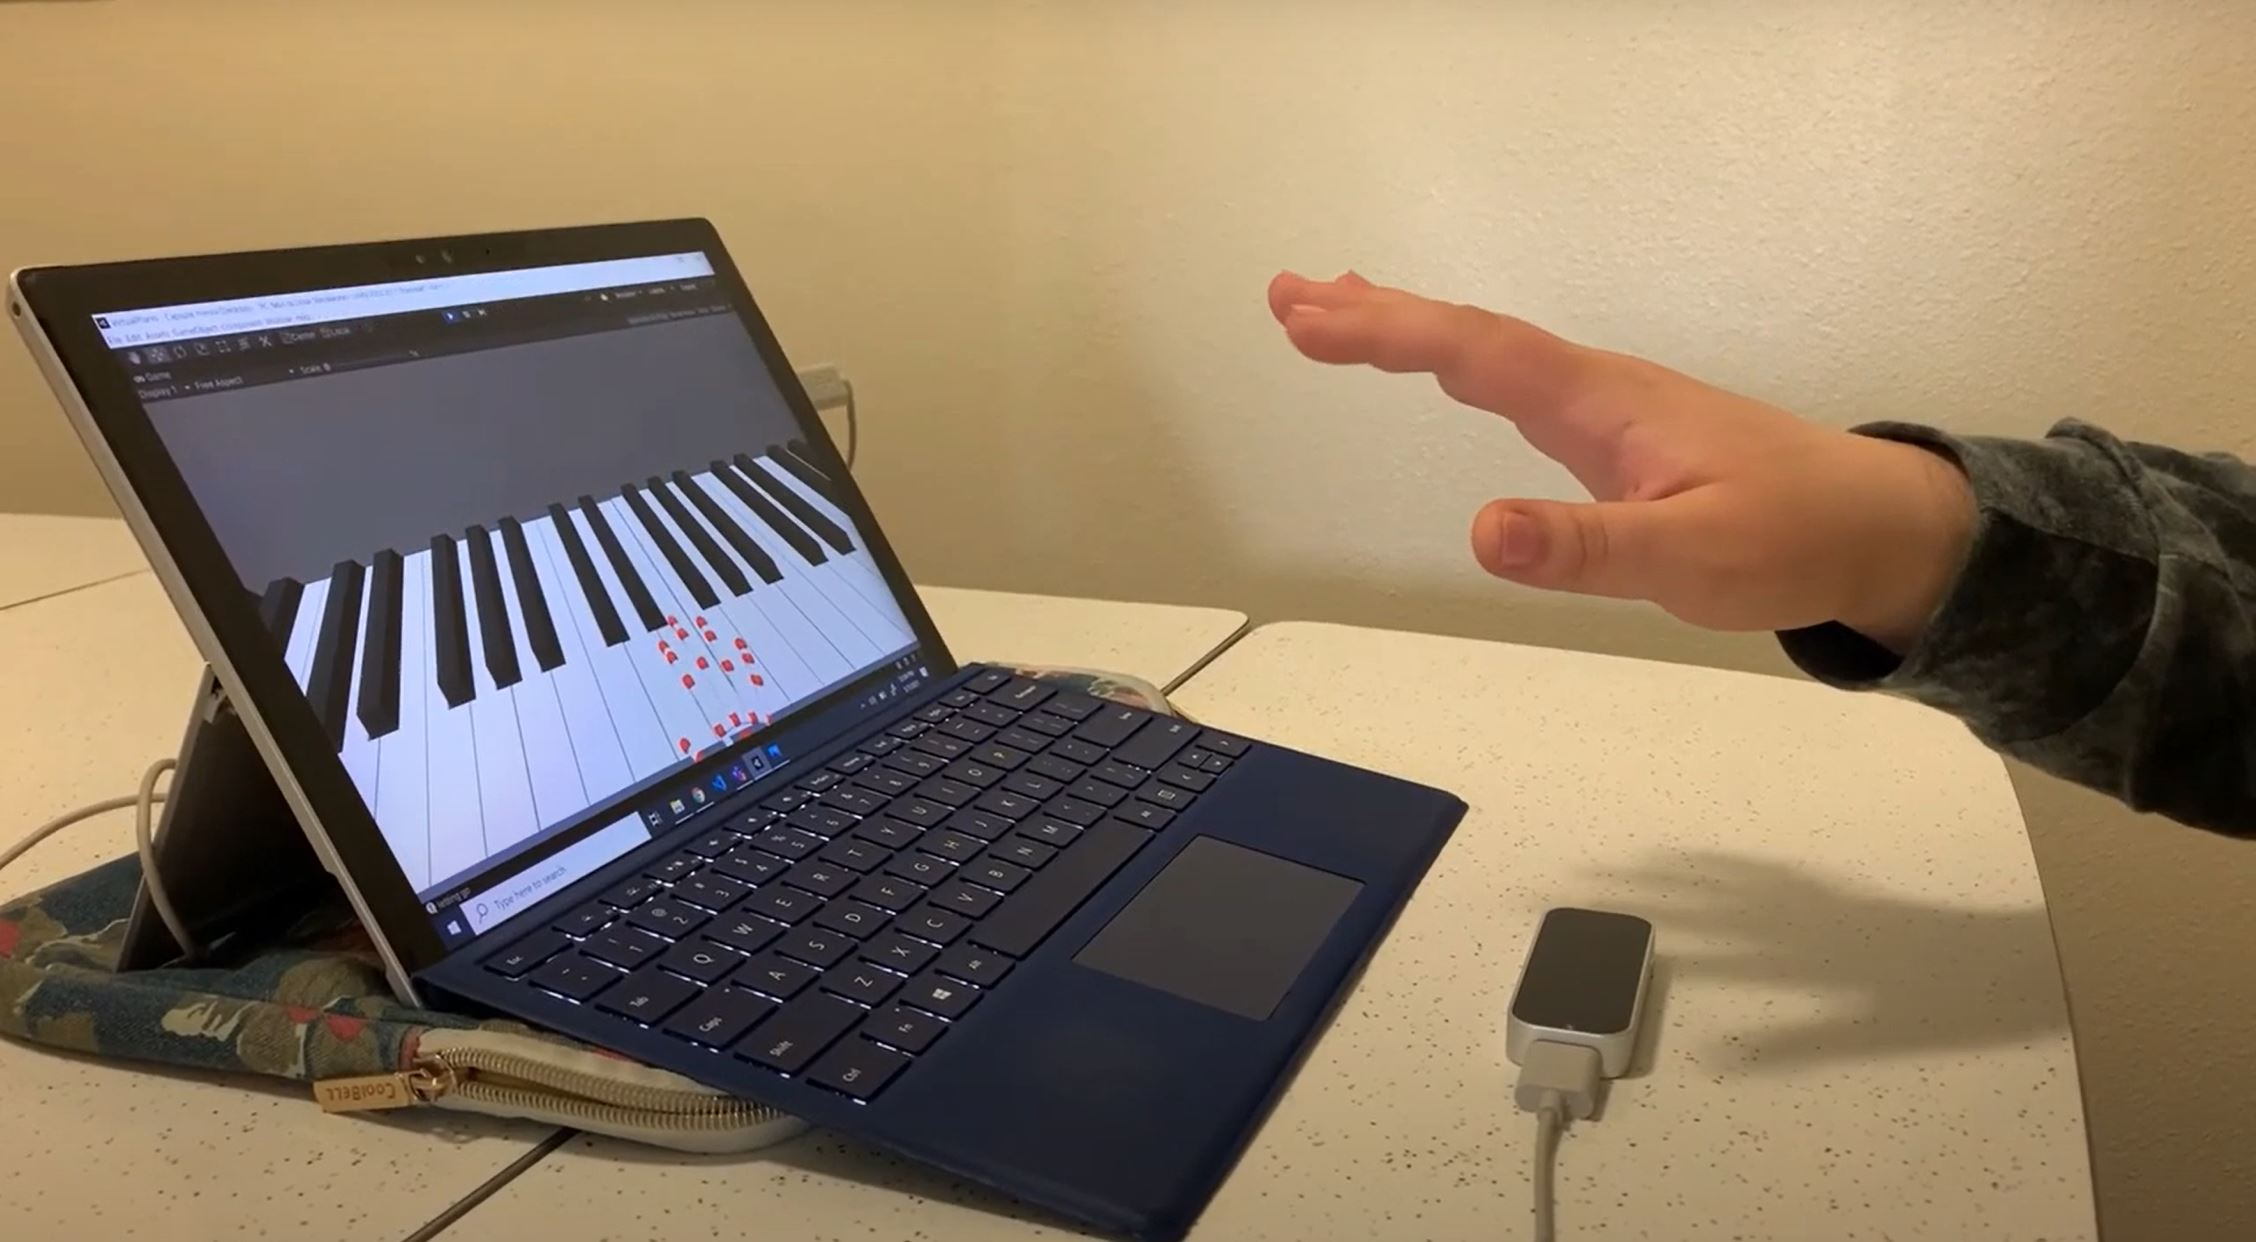
\includegraphics[width=7cm, height=4cm]{IEEEtran/VPhand.JPG}
\centering
\caption{Kopacz demonstrates the virtual piano on Unity using the Leap Motion device.}
\end{figure}

\section{Methods}
To create the virtual piano, our team adapted a piano model in Unity to virtually play the instrument using a Leap Motion device. We added the existing model, created by another team in Blender, to Unity and added additional components like the Leap Motion, lighting, and adjusted the camera to view the notes around middle C. From there, we added colliders to every key as well as capsule colliders to bone three of each finger (the tip). When a finger and key collide, a script which is attached to each key is called. We developed the script using Visual Studio Code. In the script, the audio clip for that note is played and the key is depressed. When the two are no longer colliding, the key raises back up. This allows the user to press and hold notes.

After we created the script, we attached an audio clip to each key. We were unable to find a full range of notes that were of good quality and cost effective. The piano currently has the notes from C4 to B4, chromatically. This means it has a total of 12 notes.Users of the virtual piano are able to use one or both hands, as shown in Figure 3. 

\begin{figure}[h]
\centering
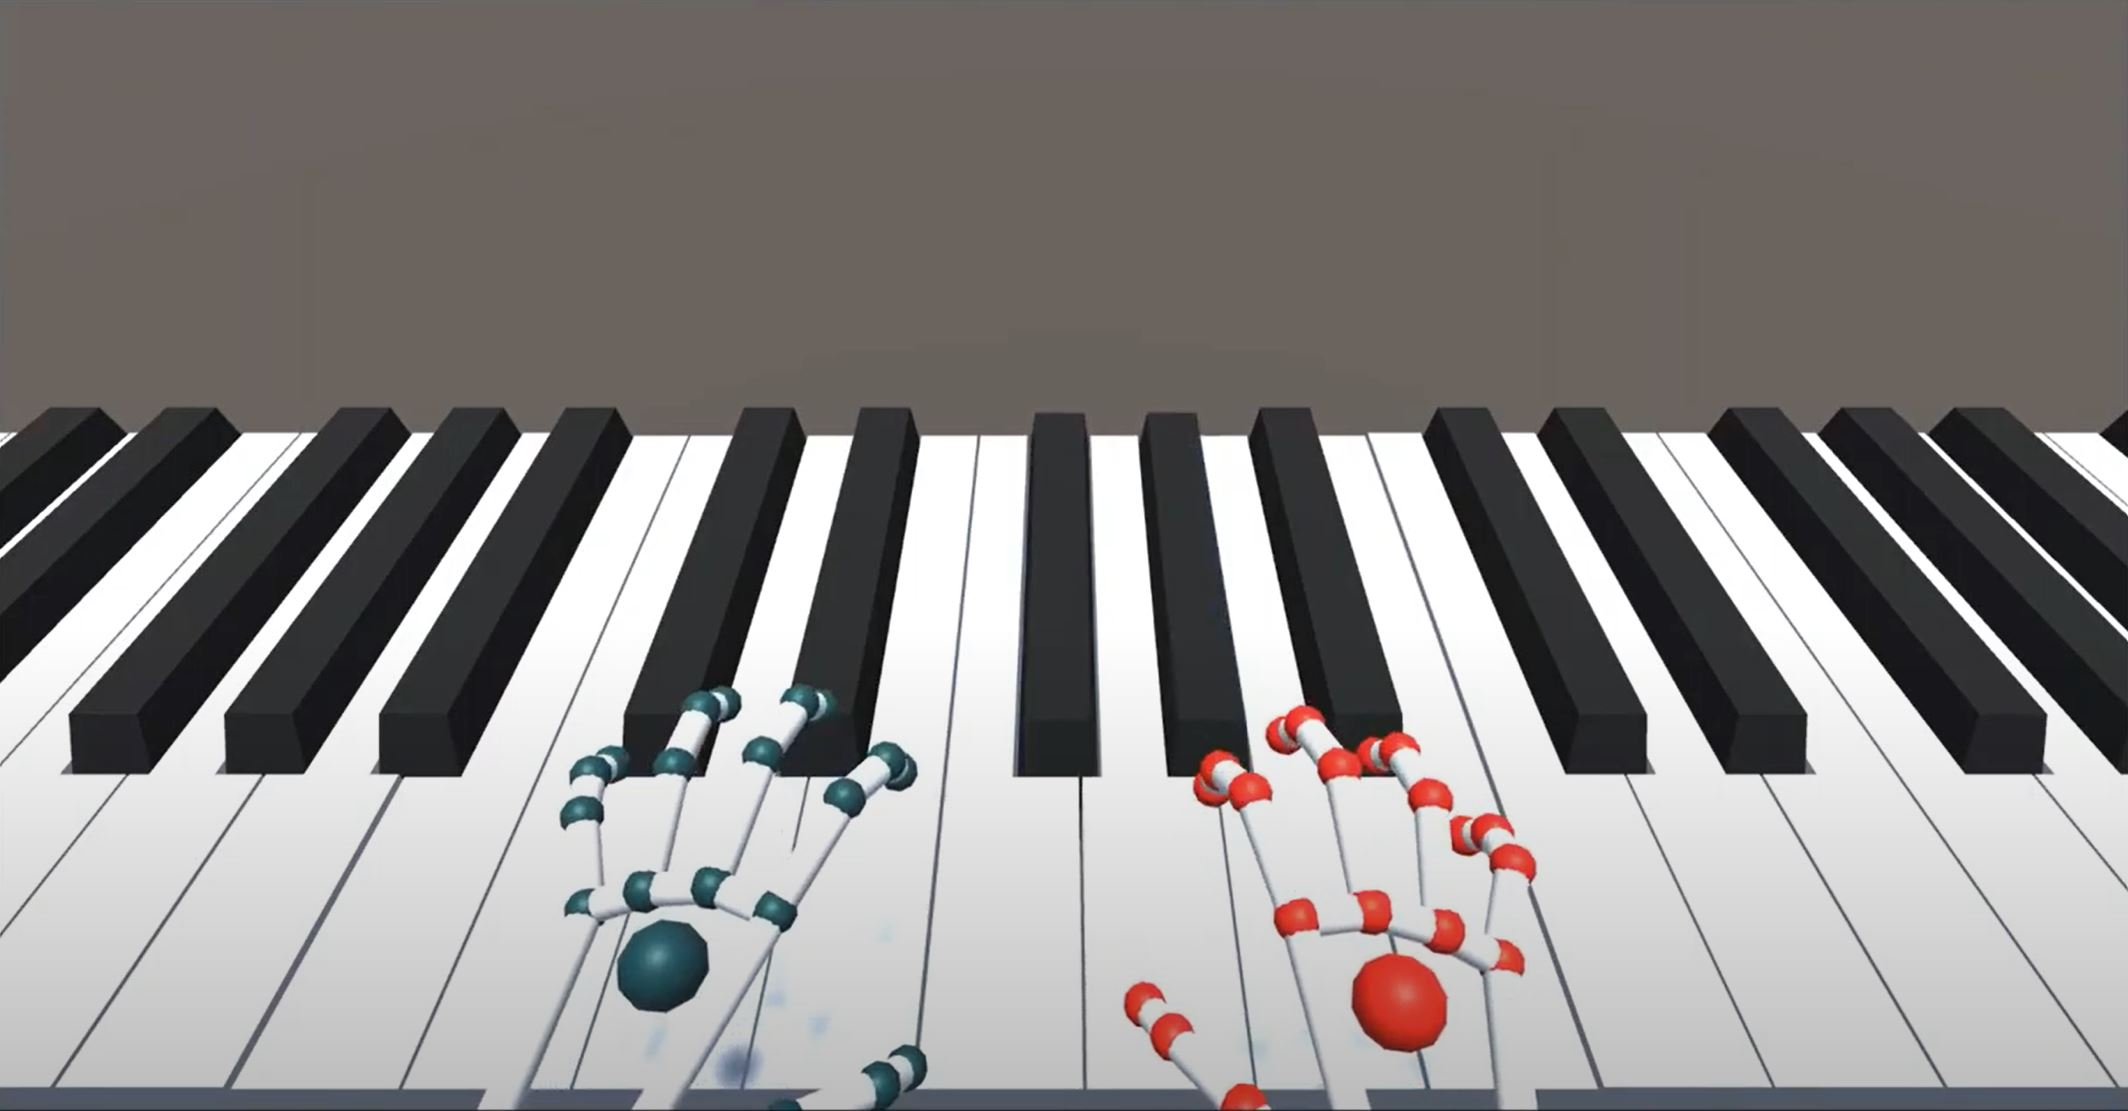
\includegraphics[width=7cm, height=4cm]{IEEEtran/UnityHands.JPG}
\centering
\caption{Virtual piano model in Unity. Image taken by Kopacz and VandeRiet.}
\end{figure}

Our repeated-measures experiment for this project allowed us to get feedback from a group of volunteers and get their opinions on the features and format. We created a survey using Google Forms to allow participants to complete the experiment while working remotely. The participants were first asked a few questions to get a feel for the demographic. Some of the questions included gender, age, career background, etc.. We also asked a few questions regarding their musical background to see how familiar the participants were with musical instruments. The participants were then asked to watch a short video we created as an overview of the project. It included an explanation to how the piano was developed and how it is played. It also featured several angles to allow the volunteers to understand as much of the project as possible. In the future, we hope to allow people to test the virtual piano in person. Next, we asked some followup questions: rate, on a scale of one to five, how close the virtual piano is to a real piano, what features is the piano missing, and what should be taken out or changed in order to improve the functionality. 

\section{Results}
The results of the survey gave us some valuable insight to improve the first prototype of the virtual piano. We found that of the 22 participants, 13 play an instrument, eight of which are the piano. This was important because it allowed us to see how the virtual piano compares to a real piano. These eight participants have extensive knowledge on the look and feel of a piano, though most people have at least touched a piano before. Close to 80\% of all of the participants believed that the virtual piano could be closer to a real piano after improvements.

\begin{figure}[h]
\centering
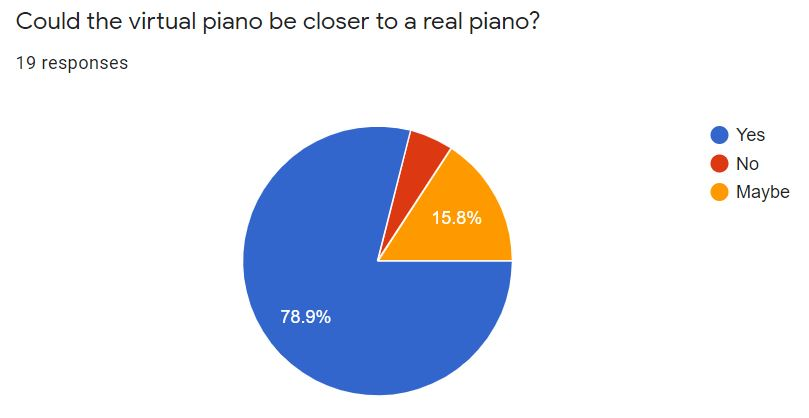
\includegraphics[width=7cm, height=4cm]{IEEEtran/Graph2.JPG}
\centering
\caption{This graph was taken from survey feedback from participants. It shows how most participants believed that after some improvements, this virtual piano could function closer to a real piano.}
\end{figure}

The main criticisms included that the virtual piano was too sensitive, and that the accuracy needed to be improved. Due to the high sensitivity, it is not uncommon for multiple keys to be pressed at the same time. The Leap Motion sensor is not as accurate as this virtual instrument requires, and that could be a feature that is improved in the future. 

Additionally, adding a sustain pedal was suggested by multiple participants, which could allow for longer notes, although more sensors or hardware would be necessary. Several people also stated that to play a piano well, it requires haptic feedback to allow them to play the correct notes without looking. While the Leap Motion Sensor does not have this capability, it is possible that another technology could allow this feature.

Overall, the participants thought that the current features of the virtual piano were necessary and should be kept, although the suggestions previously mentioned should be added eventually as improvements.

\section{Limitations of Study}
This virtual piano is rather simple to use, and easy to understand. However, there are plenty of limitations. The primary limitation is that users must know how to play the piano, or at least be familiar with one. It would be a challenge to play a more complicated piece of music on this virtual piano, due to its sensitivity, however upon improvements, it could certainly be possible. 

Another limitation is that the program that was created cannot currently work with other virtual instruments. A virtual violin, guitar, or flute, for example, would all require completely different 3D models and programs started from scratch.

It would be possible to use a different sensor, rather than the Leap Motion, in order to attempt to decrease sensitivity, but it is likely that parts of the program would have to be rewritten. However, a sensor with less sensitivity and a more precise range would help improve the functionality of the virtual piano greatly.


\section{Design Implications}
With the current design and program, the development of the virtual piano is far from over. Currently, the best way to "play" the program is to use one's pointer finger to virtually touch the keys. Users simply hover their hands over the device and use their fingers to press down keys. When the user's finger moves down, the leap motion tracks this movement and presses a key down on the screen. Due to the inaccuracy of the Leap Motion tool, the program can mistake additional fingers also pressing down keys. This means keys next to the desired key are often times also played. When using two hands, the program can also struggle to see both hands clearly. When the user is primarily focused on one hand, the other hand has the potential to glitch. While using one finger is an easy way to get around these issues, the program was designed for the user to use both hands and every finger, just like they would with a real piano.

\begin{figure}[h]
\centering
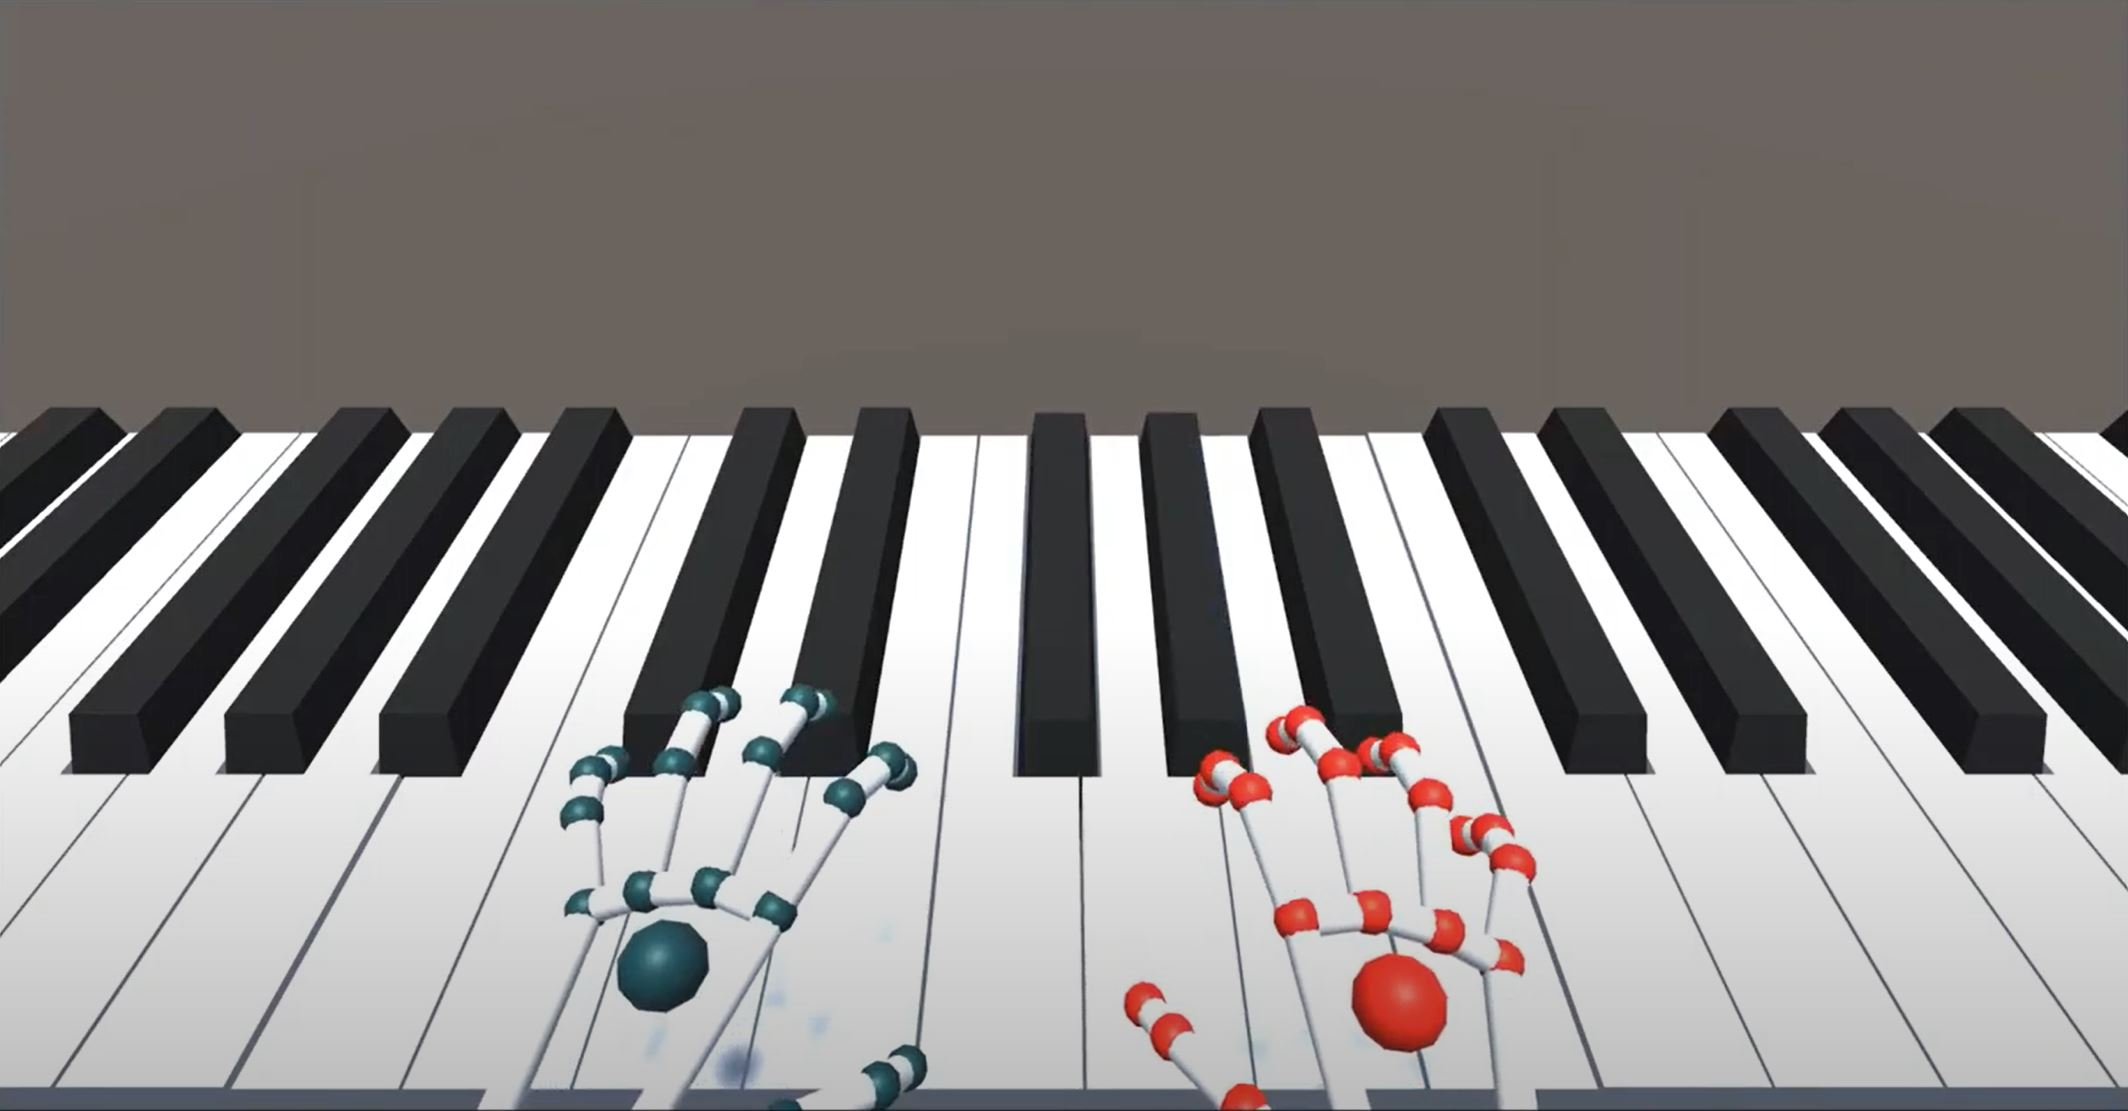
\includegraphics[width=7cm, height=4cm]{IEEEtran/UnityHands.JPG}
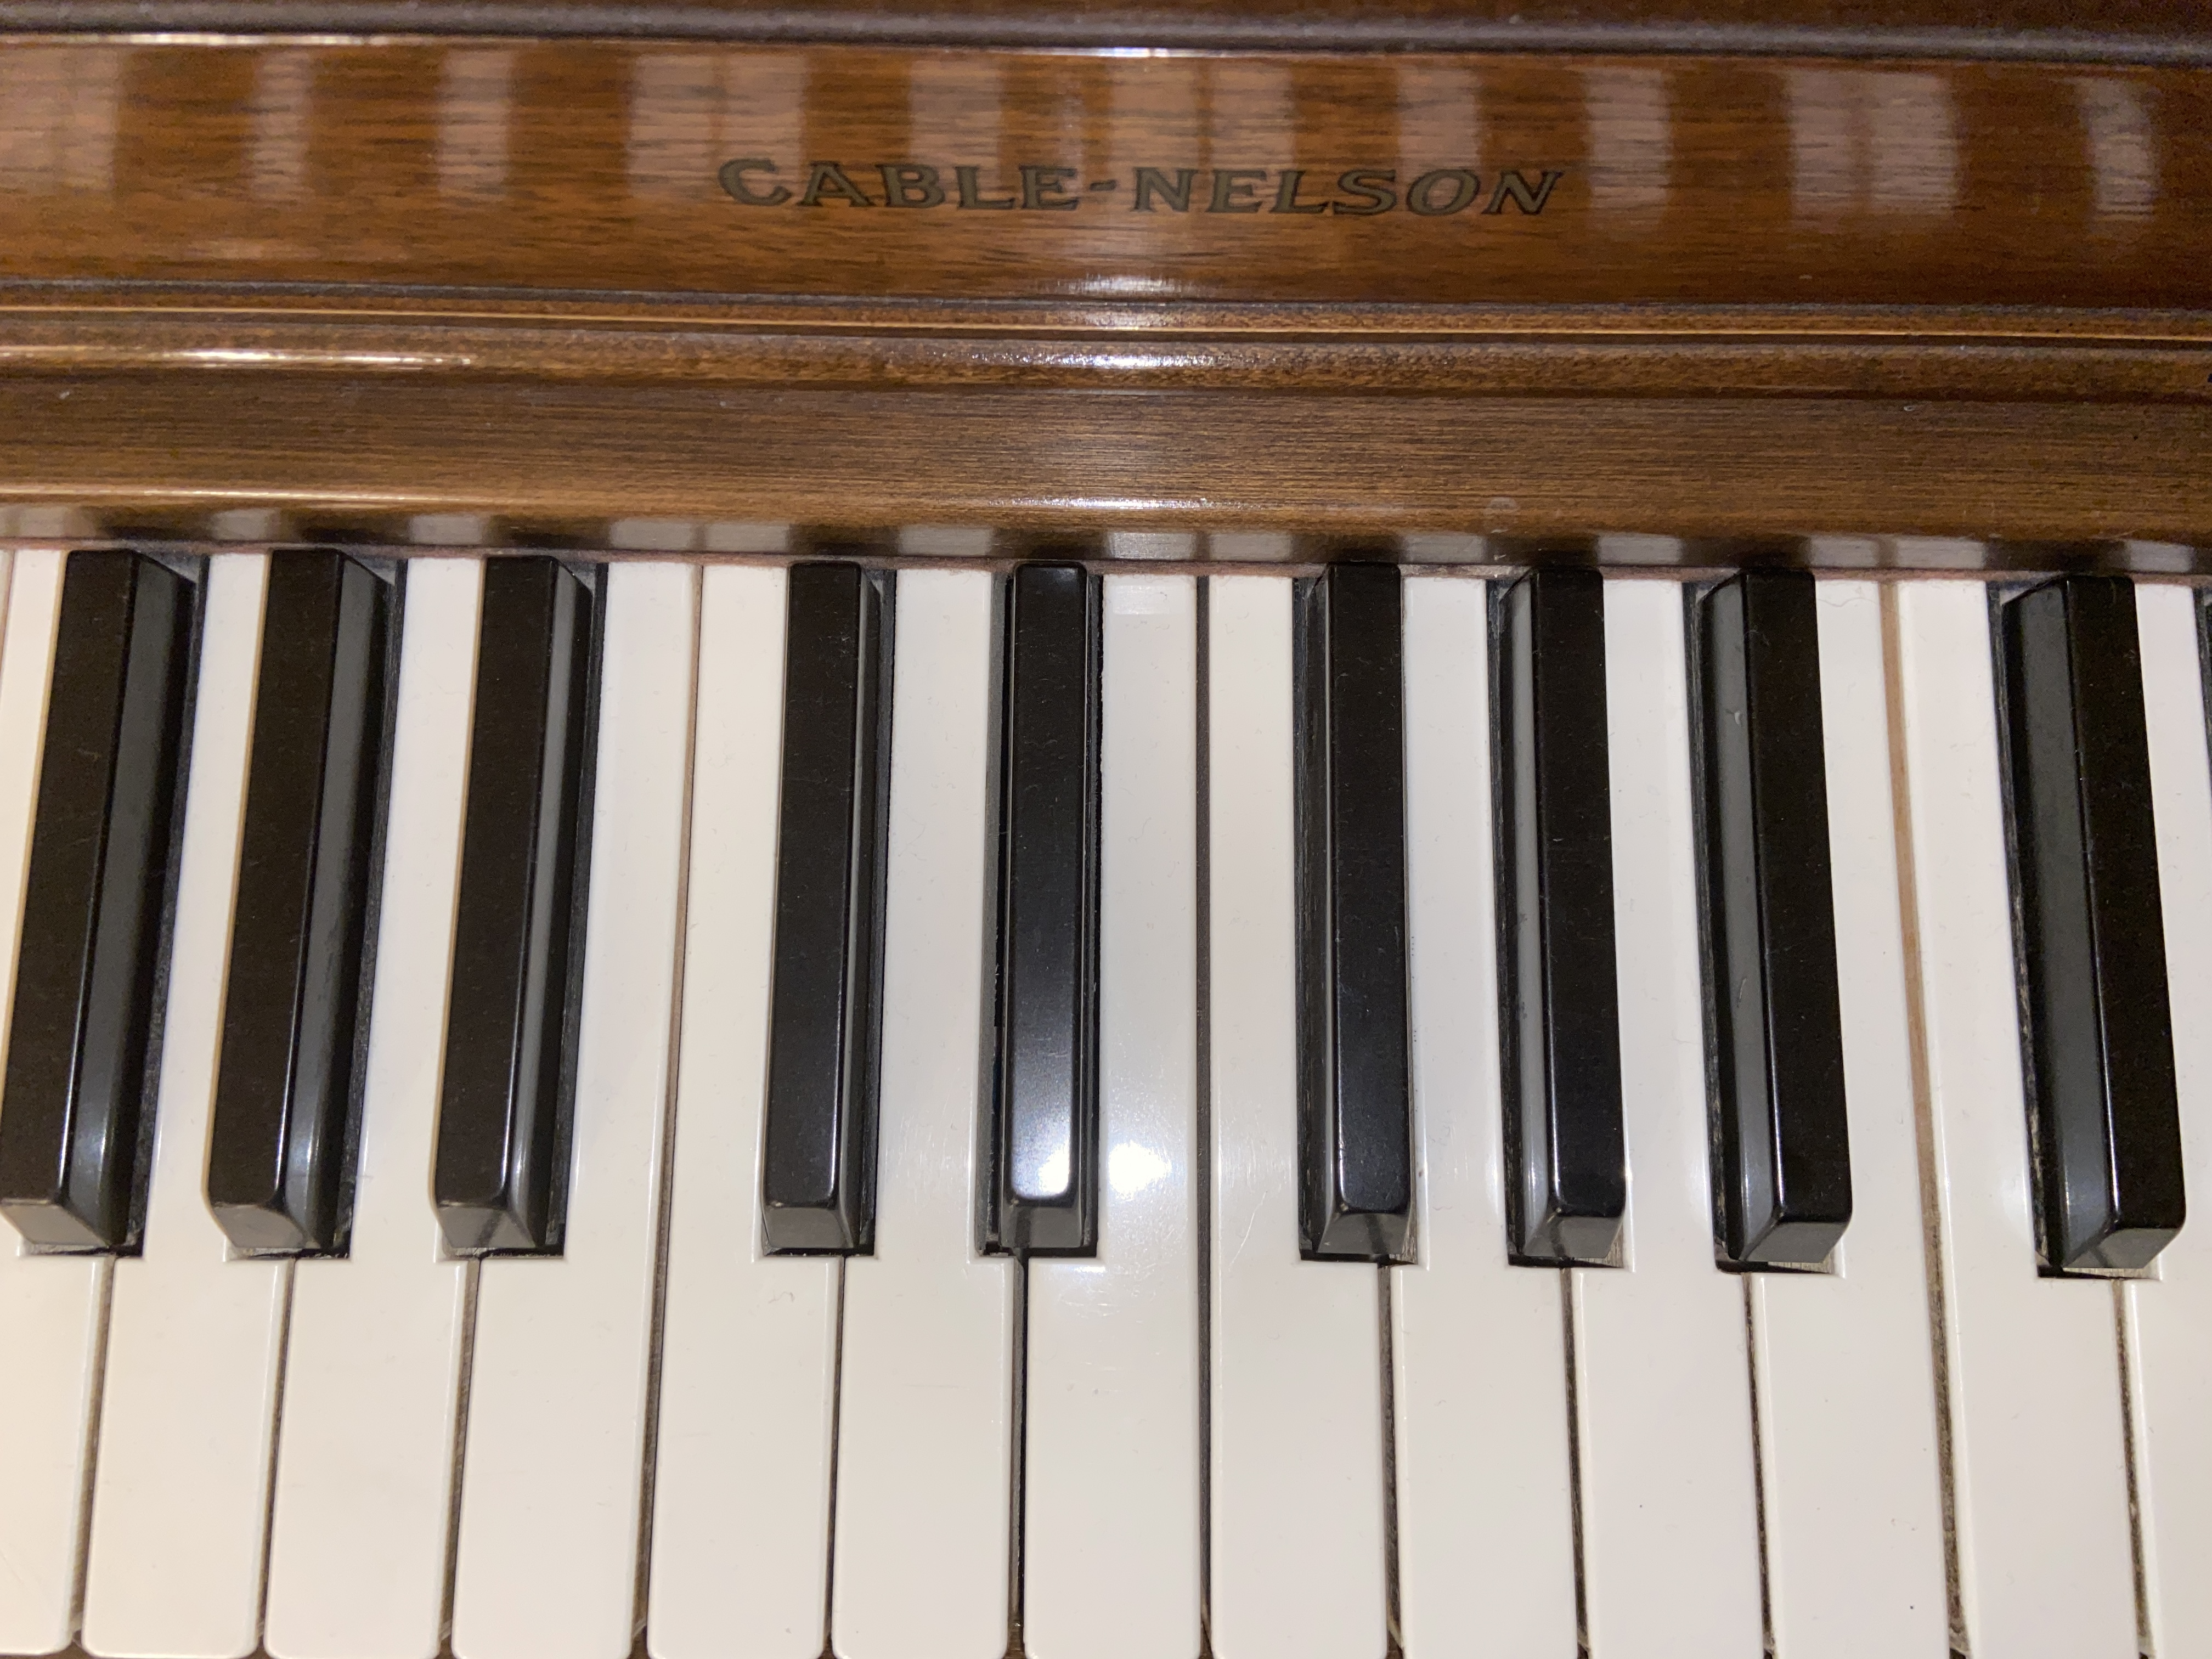
\includegraphics[width=7cm, height=4cm]{IEEEtran/IMG_9837.JPG}
\centering
\caption{Figure 4 (top) is shown again with a comparison to the keys of a real piano (bottom). Both images taken by Kopacz and VandeRiet.}
\end{figure}

\section{Conclusion and Future Work}
Future research regarding virtual reality musical instruments could include the composition of music virtually. There are systems that are able to “compose music reflecting users’ feeling of music,” [17]. This could aim to produce music virtually through the use of systems such as the Leap Motion. 

Additionally, adding more audio clips to correspond with more octaves would be another improvement for the virtual piano. Even further, changing the volume based on how fast the key is played could be incorporated. Currently, when a user virtually holds a key down or just lightly taps it, the sound is the same. Upon this improvement, the collision function would be able to track the magnitude of collision and play the corresponding audio clip at a certain volume for each magnitude type.

Also, virtual reality musical instruments are the future of adaptive music technology. “Adaptive music technology refers to digital technologies allowing people who cannot play traditional musical instruments to engage in musical activities, without external sources assisting in the music making,” [4]. Virtual reality musical instruments have played an important part in the development of human computer interaction and have the potential to contribute to adaptive music technology and other developments in the future.

Overall, the project was a success. We started with just the 3D model of the piano, and were able to add all of the components to create a working prototype of a virtual piano that can be played using a Leap Motion. As this is a prototype, there are a multitude of potential improvements that could make this piano even better. Although many features could be added to this project, the foundations we have created are a good base for us and others to build upon in the future. The virtual piano itself needs plenty of improvements, but it is functional and exceeded our team's expectations.

\section*{Acknowledgements}
The authors of this paper would like to thank Justin Kopacz for his contributions to the project. Kopacz is a Principal AI Software Engineer at Northrop Grumman and his efforts have contributed to the success of the project. 

We would also like to thank Desarae Cruz, Edward Lee, and Trey Yu for creating the model of the piano in CS464 for their project during a previous semester of the class. 

Thank you to our survey participants, including, Samuel Bazen, Cory Dahn, Mari Dudek, Zachary Geauthreaux, Tor Larson, and Wes Wallace who are our fellow CS464 students.

Finally, we would like to thank our CS464 professor Francisco Ortega, Ph.D, for our inspiration and providing us with the Leap Motion tool and other resources to complete this project.



% trigger a \newpage just before the given reference
% number - used to balance the columns on the last page
% adjust value as needed - may need to be readjusted if
% the document is modified later
%\IEEEtriggeratref{8}
% The "triggered" command can be changed if desired:
%\IEEEtriggercmd{\enlargethispage{-5in}}

% references section

% can use a bibliography generated by BibTeX as a .bbl file
% BibTeX documentation can be easily obtained at:
% http://mirror.ctan.org/biblio/bibtex/contrib/doc/
% The IEEEtran BibTeX style support page is at:
% http://www.michaelshell.org/tex/ieeetran/bibtex/
%\bibliographystyle{IEEEtran}
% argument is your BibTeX string definitions and bibliography database(s)
%\bibliography{IEEEabrv,../bib/paper}
%
% <OR> manually copy in the resultant .bbl file
% set second argument of \begin to the number of references
% (used to reserve space for the reference number labels box)
\begin{thebibliography}{1}


\bibitem{IEEEhowto:Bachmann}
D.~Bachmann, F.~Weichert, and G.~Rinkenauer, \emph{Review of Three-Dimensional Human-Computer Interaction with Focus on the Leap Motion Controller.}.\hskip 1em plus
  0.5em minus 0.4em\relax Sensors 18.7 (2018): 2194. Crossref. Web. \usepackage{hyperref}
  \url{https://www.mdpi.com/1424-8220/18/7/2194}.
  
\bibitem{IEEEhowto:Brown}
D.~Brown,et al., \emph{Leimu: Gloveless Music Interaction Using a Wrist Mounted Leap Motion.}.\hskip 1em plus
  0.5em minus 0.4em\relax July 2016,
  \usepackage{hyperref} \url{www.researchgate.net/publication/310699028\_Leimu\_Gloveless\_Music\_Interaction\_Using\_a\_Wrist\_Mounted\_Leap\_Motion}.
  
\bibitem{IEEEhowto:Wijaya}
F.~Wijaya, Y.~Tsenf, W.~Tsai, T.~Pan, and M.~Hu, \emph{VR Piano Learning Platform with Leap Motion and Pressure Sensors}.\hskip 1em plus
  0.5em minus 0.4em\relax 2020 IEEE Conference on Virtual Reality and 3D User Interfaces Abstracts and Workshops (VRW), Atlanta, GA, USA, 2020, pp. 584-585, doi: 10.1109/VRW50115.2020.00143. Retrieved from: 
  \usepackage{hyperref} \url{https://ieeexplore.ieee.org/abstract/document/9090628}.
  
\bibitem{IEEEhowto:Frid}
E.~Frid, \emph{Accessible Digital Musical Instruments - A Survey of Inclusive Instruments Presented at the NIME, SMC and ICMC Conferences}.\hskip 1em plus
  0.5em minus 0.4em\relax Retrieved from: 
  \usepackage{hyperref} \url{https://www.researchgate.net/profile/Emma-Frid-2/publication/327187266\_Accessible\_Digital\_Musical\_Instruments\_-\_A\_Survey\_of\_Inclusive\_Instruments\_Presented\_at\_the\_NIME\_SMC\_and\_ICMC\_Conferences/links/5b8688e292851c1e12392697/Accessible-Digital-Musical-Instruments-A-Survey-of-Inclusive
  -Instruments-Presented-at-the-NIME-SMC-and-ICMC-Conferences.pdf}.
  
\bibitem{IEEEhowto:Han}
J.~Han, and N.~Gold, \emph{Lessons Learned in Exploring the Leap Motion™ Sensor for Gesture-based Instrument Design}.\hskip 1em plus
  0.5em minus 0.4em\relax 2014. Retrieved from: 
  \usepackage{hyperref} \url{https://discovery.ucl.ac.uk/id/eprint/1436807/}.
  
\bibitem{IEEEhowto:Holland}
S.~Holland, K.~Wilkie, P.~Mulholland, and A.~Seago, \emph{Music interaction: understanding music and human-computer interaction}.\hskip 1em plus
  0.5em minus 0.4em\relax 2013. In: Holland, Simon; Wilkie, Katie; Mulholland, Paul and Seago, Allan eds. Music and Human-Computer Interaction. Cultural Computing. London: Springer, pp. 1-36. 
  
\bibitem{IEEEhowto:Li}
~Li, \emph{Application of Augmented Reality Technology in Piano Teaching System Design.}.\hskip 1em plus
  0.5em minus 0.4em\relax Educational Sciences: Theory & Practice, vol. 18, no. 5, Oct. 2018, pp. 1712–1721. EBSCOhost, doi:10.12738/estp.2018.5.070.
 
\bibitem{IEEEhowto:Liang}
H.~Liang, et al., \emph{Barehanded Music: Real-time Hand Interaction for Virtual Piano.}.\hskip 1em plus
  0.5em minus 0.4em\relax 08 November 2017, Proceedings of the 20th ACM SIGGRAPH Symposium on Interactive 3D Graphics and Games. 
  \usepackage{hyperref} \url{https://www.researchgate.net/publication/291831744\_Barehanded\_Music\_Real-time\_Hand\_Interaction\_for\_Virtual\_Piano}.
  
\bibitem{IEEEhowto:Miller}
J.~Miller, and T.~Hammond, \emph{Wiiolin: a virtual instrument using the Wii remote}.\hskip 1em plus
  0.5em minus 0.4em\relax 2010. Proceedings of the 2010 Conference on New Interfaces for Musical Expression (NIME 2010), Sydney, Australia. Retrieved from 
  \usepackage{hyperref} \url{https://www.researchgate.net/publication/228414838\_Wiiolin\_a\_virtual\_instrument\_using\_the\_Wii\_remote}.
  
\bibitem{IEEEhowto:Montag}
M.~Montag, S.~Sullivan, S.~Dickey, and C.~Leider, \emph{A Low-Cost, Low-Latency Multi-Touch Table with Haptic Feedback for Musical Applications.}.\hskip 1em plus
  0.5em minus 0.4em\relax 2011. Proceedings of the International Conference on New Interfaces for Musical Expression, (June), 8–13. Retrieved from  
  \usepackage{hyperref} \url{https://www.nime.org/proceedings/2011/nime2011\_008.pdf}.
  
\bibitem{IEEEhowto:Malloch}
J.~Malloch, D.~Birnbaum, E.~Sinyor, and M.~Wanderley, \emph{Towards a New Conceptual Framework for Digital Musical Instruments.}.\hskip 1em plus
  0.5em minus 0.4em\relax 2006. Proceedings of the 9th International Conference on Digital Audio Effects (pp. 49–52). Retrieved from   
  \usepackage{hyperref} \url{http://www.dafx.ca/proceedings/papers/p\_049.pdf}.
  
\bibitem{IEEEhowto:Hariadi}
R.R.~Hariadi, and I.~Kuswardayan, \emph{Design and implementation of Virtual Indonesian Musical Instrument (VIMi) application using Leap Motion Controller}.\hskip 1em plus
  0.5em minus 0.4em\relax 2016 International Conference on Information & Communication Technology and Systems (ICTS), Surabaya, Indonesia, 2016, pp. 43-48, doi: 10.1109/ICTS.2016.7910270. Retrieved from 
  \usepackage{hyperref} \url{https://ieeexplore.ieee.org/abstract/document/7910270}.
  
\bibitem{IEEEhowto:Ritter}
M.~Ritter, and A.~Aska, \emph{Leap Motion As Expressive Gestural Interface}.\hskip 1em plus
  0.5em minus 0.4em\relax 2014. Retrieved from 
  \usepackage{hyperref} \url{http://smc.afim-asso.org/smc-icmc-2014/papers/images/VOL\_1/0659.pdf}.
  
\bibitem{IEEEhowto:Salz}
D.~Salz, and F.~Azam, \emph{Playing a Virtual Piano with Dynamics.}.\hskip 1em plus
  0.5em minus 0.4em\relax 2019. Retrieved from 
  \usepackage{hyperref} \url{stanford.edu/class/ee267/Spring2019/report_azam.pdf}.
  
\bibitem{IEEEhowto:Serafin}
S.~Serafin, et al., \emph{Virtual Reality Musical Instruments: State of the Art, Design Principles, and Future Directions.}.\hskip 1em plus
  0.5em minus 0.4em\relax Computer Music Journal, vol. 40, no. 3, 2016, pp. 22–40., doi:10.1162/comj\_a\_00372. 
  
\bibitem{IEEEhowto:Silva}
E.S.~Silva, J.~Abreu, J.H.~Almeida, V.~Teichrieb, and G.~Ramalho, \emph{A Preliminary Evaluation of the Leap Motion Sensor as Controller of New Digital Musical Instruments.}.\hskip 1em plus
  0.5em minus 0.4em\relax 2013. Retrieved from 
  \usepackage{hyperref} \url{http://compmus.ime.usp.br/sbcm/2013/pt/docs/art\_tec\_1.pdf}.
  
\bibitem{IEEEhowto:Unehara}
M.~Unehara, and T.~Onisawa, \emph{Music Composition by Interaction between Human and Computer.}.\hskip 1em plus
  0.5em minus 0.4em\relax New Generation Computing, vol. 23, no. 2, Apr. 2005, pp. 181–191. EBSCOhost, doi:10.1007/BF03037494.
  
\bibitem{IEEEhowto:Yan}
L.~Yan, et al., \emph{Design of Piano Teaching System Based on Internet of Things Technology.}.\hskip 1em plus
  0.5em minus 0.4em\relax Journal of Intelligent & Fuzzy Systems, vol. 37, no. 5, Nov. 2019, pp. 5905–5913. EBSCOhost, doi:10.3233/JIFS-179172. Retrieved from 
  \usepackage{hyperref} \url{https://web-b-ebscohost-com.ezproxy2.library.colostate.edu/ehost/detail/detail\?vid=27\&sid=ecfdc204-494e-40fc-b7d0-9aeba2d8b0df\%40pdc-v-sessmgr03\&bdata=JkF1dGhUeXBlPWNvb2tpZSxpcCx1cmwsY3BpZCZjdXN0aWQ9czQ2NDA3OTImc2l0ZT1laG9zdC1saXZl\#AN=139809124\&db=aph}.
  
  \bibitem{IEEEhowto:Burdea}
G.~Burdea, \emph{Key Note Address: Virtual Rehabilitation Benefits and Challenges.}.\hskip 1em plus
  0.5em minus 0.4em\relax Rutgers University, 2006. Retrieved from
  \usepackage{hyperref} \url{www.ti.rutgers.edu/publications/papers/2002\_vrmhr\_burdea.pdf}.
  


\end{thebibliography}
% that's all folks
\end{document}


